\chapter{Questionnaire}
\label{app:Questionnaire}

This section demonstrates---as an example---how to include an external PDF
document in your own \latex manuscript. This problem arises relatively often, 
\eg, in connection with questionnaires that one has created and/or used in
the thesis. Therefore, exactly this case is shown here.%
\footnote{With a nice questionnaire of the \emph{Upper Austrian Energy Saving
Association} (\url{https://www.energiesparverband.at/}).} 
It is important that the \emph{page formatting} of the own document is not
disrupted and the \emph{page numbering} correctly considers the inserted
pages.


\section{The \texttt{pdfpages} Package}

The \latex\ package \texttt{pdfpages}%
\footnote{\url{https://ctan.org/pkg/pdfpages}}
is (currently) the only option for this purpose. It is loaded automatically
by \nolinkurl{hgb.sty} with
%
\begin{LaTeXCode}[numbers=none]
\RequirePackage{pdfpages}
\end{LaTeXCode}
%
The included PDF document (a two-page questionaire) is located in
\nolinkurl{images/fragebogen.pdf}. To include all (2) pages of the PDF file
in the current document, we use the instruction
%
\begin{LaTeXCode}[numbers=none]
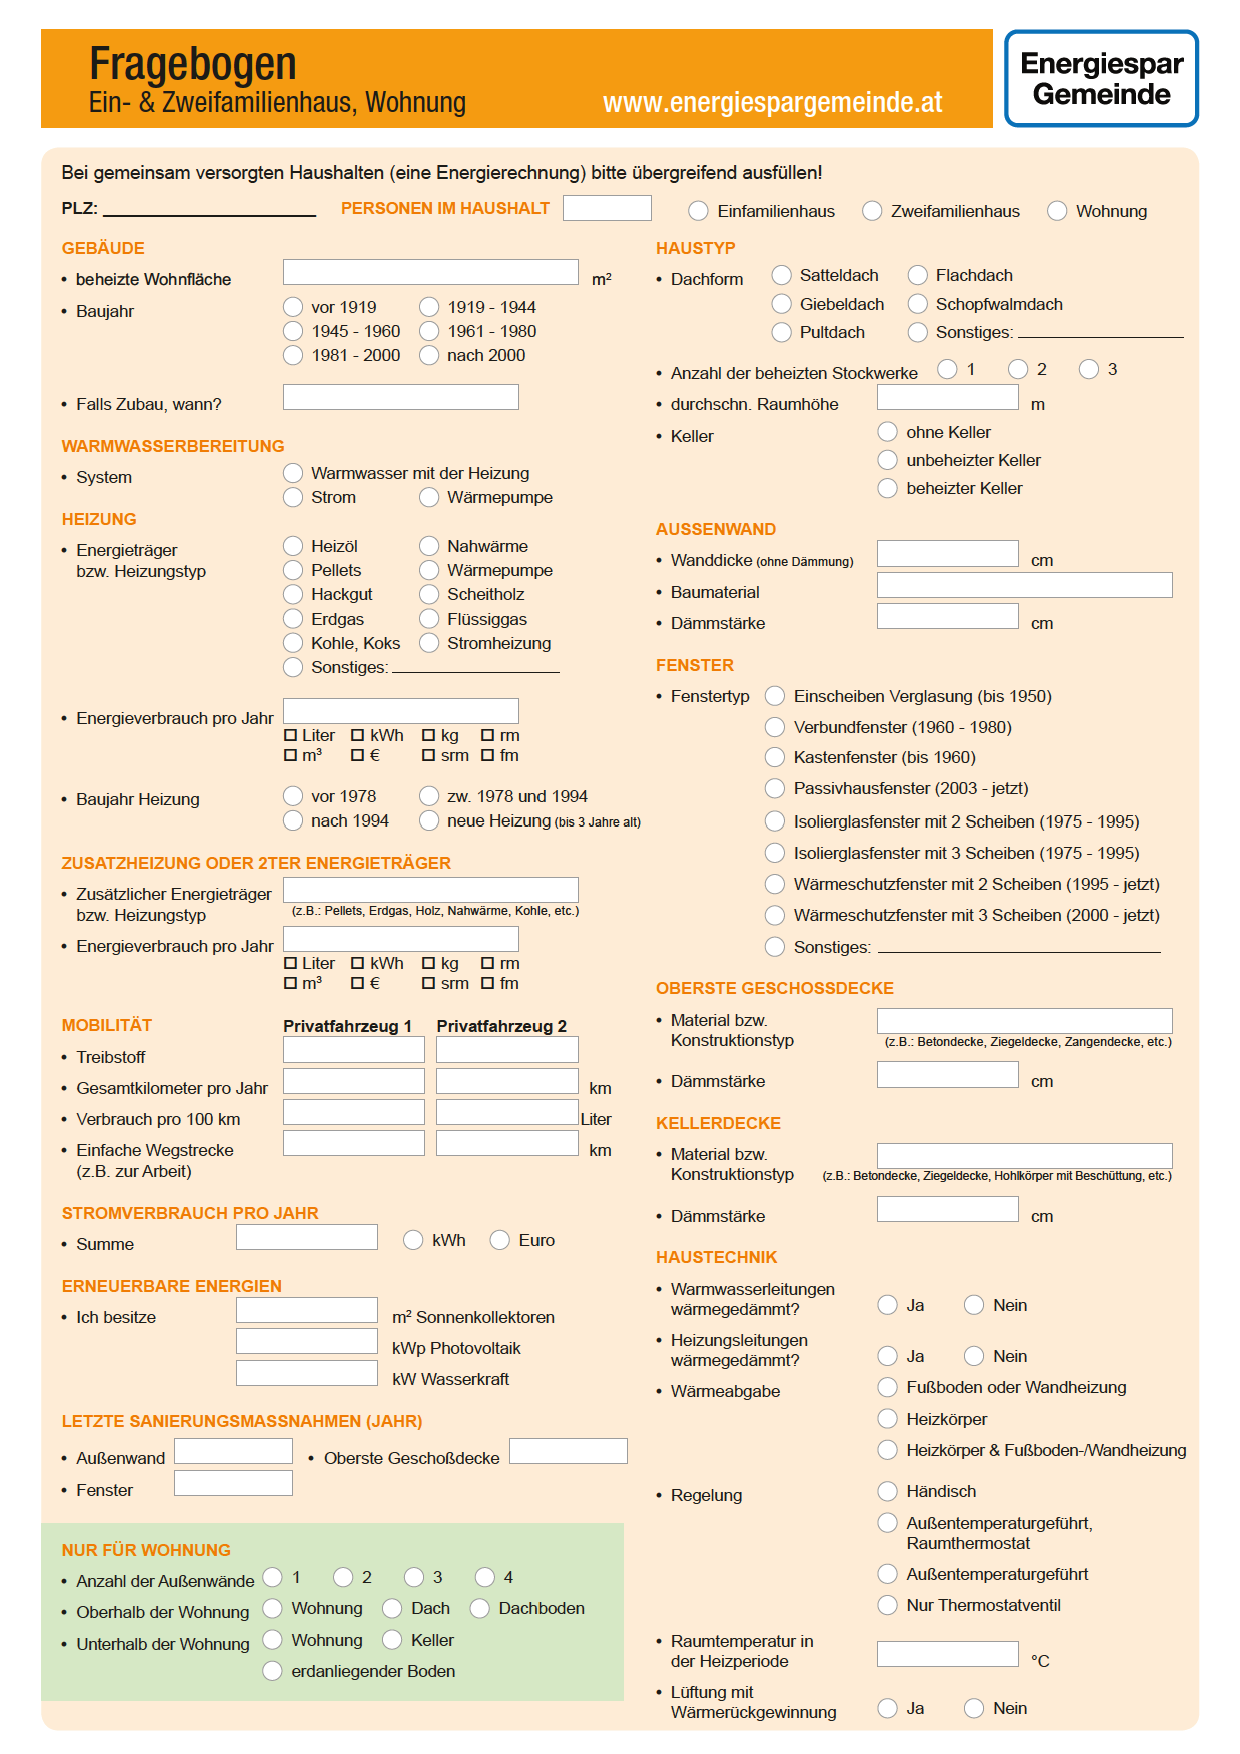
\includepdf[pages=1-,width=\textwidth,frame=true,pagecommand={}]{images/fragebogen}
\end{LaTeXCode}
%
The included pages are automatically scaled to the text width of the \latex document
by \verb!width=\textwidth! and \verb!frame=true! adds a surrounding border.

This example assumes that the external PDF document is in A4 page format.
With other formats you may have to adjust the scaling "manually" if the pages become
too tall (\eg, with \verb!width=0.9\textwidth!).

It is also important that all \emph{fonts} used in the external PDF document are
correct and fully \emph{embedded}, otherwise the PDF document generated by \latex may
not be viewable in another system environment!


\section{References to Included PDF Pages}

If you want to refer to specific pages in the included PDF, the easiest way is to import
single pages one by one and add a \emph{label} to each, as in this example:
%
\begin{LaTeXCode}[numbers=none]
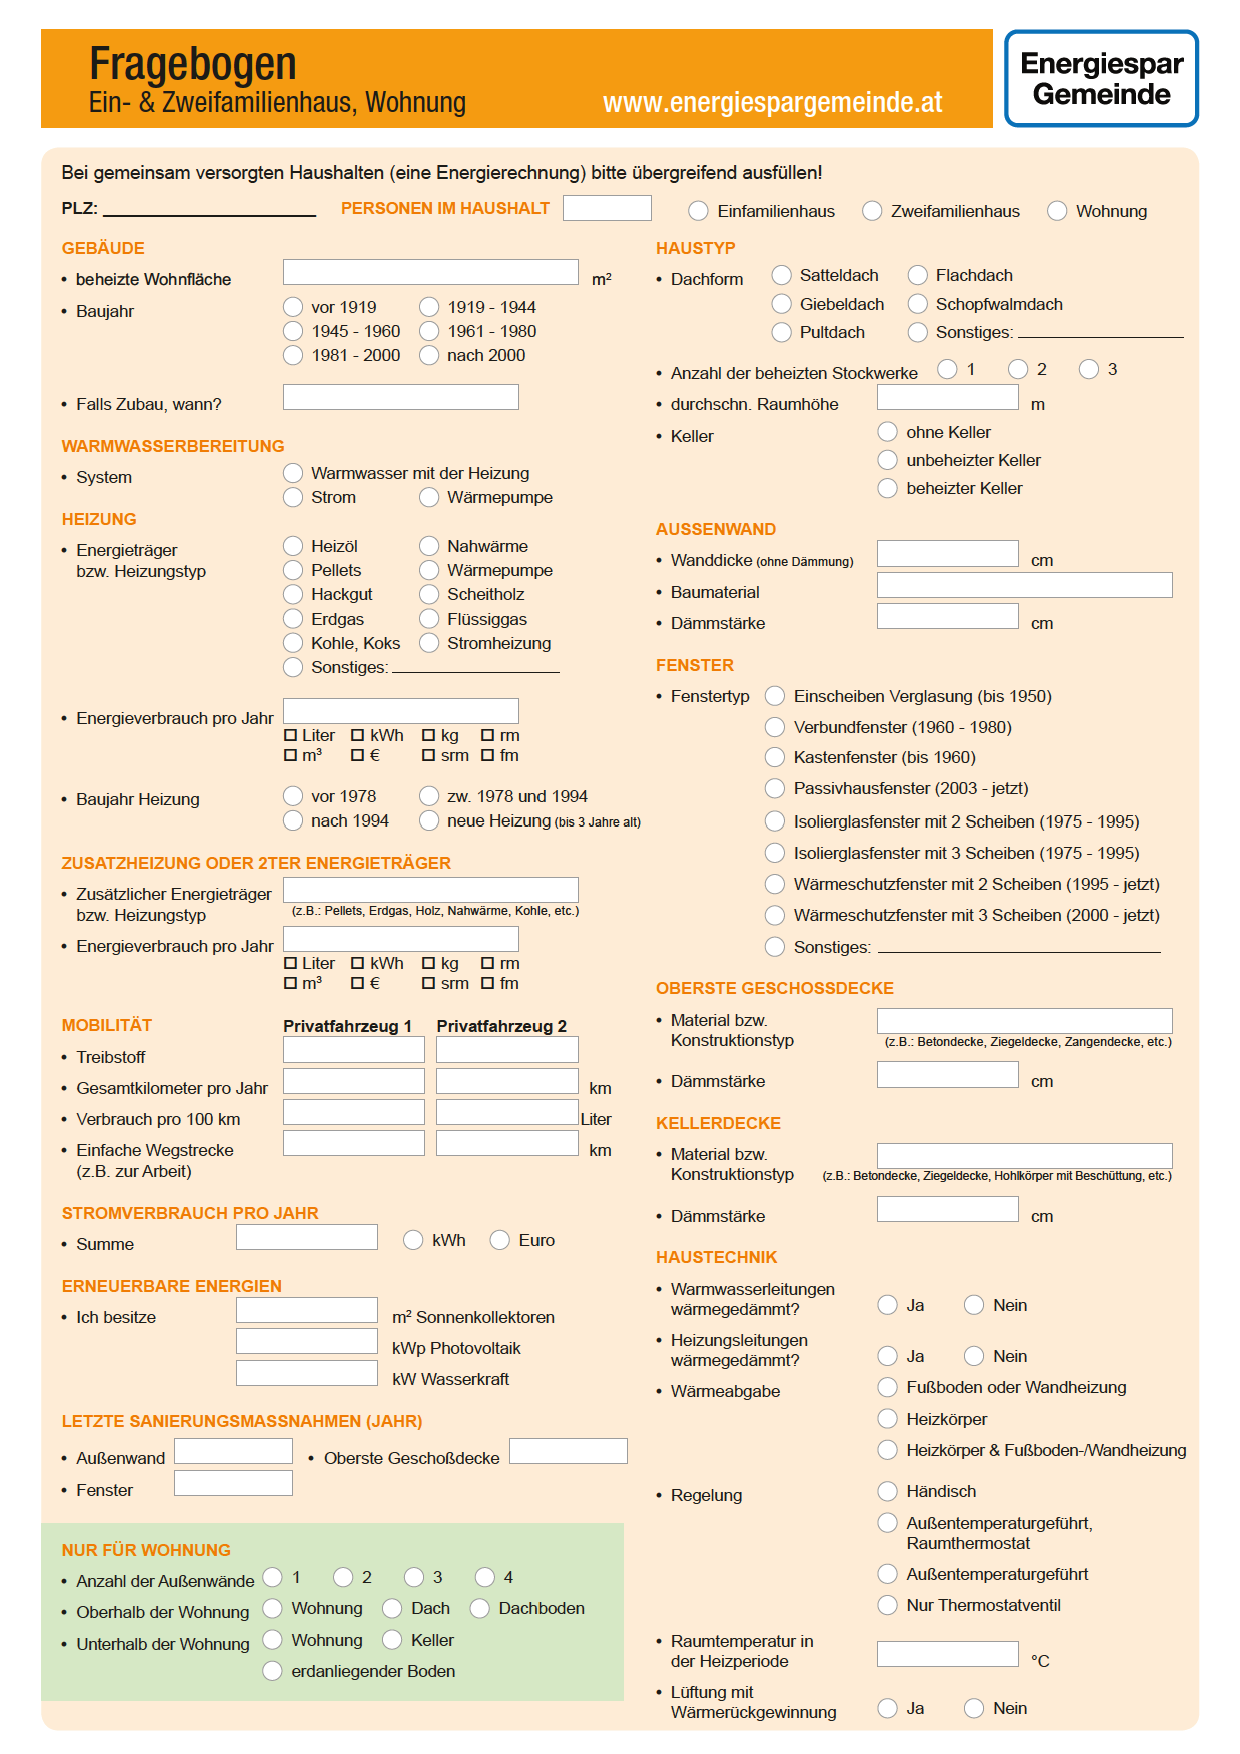
\includepdf[pages=1,width=\textwidth,frame=true,
		pagecommand={\label{PDF1}}]{images/fragebogen}
\includepdf[pages=2,width=\textwidth,frame=true,
		pagecommand={\label{PDF2}}]{images/fragebogen}
\end{LaTeXCode}
%
For example, in this case you could use \verb!\pageref{PDF2}! to specify the current page
number of the 2\textsuperscript{nd} page of the included PDF document. 
Many other options (\eg, specifying page intervals) can be found in the detailed documentation
for the \texttt{pdfpages} package.

% And here the foreign PDF document actually included:
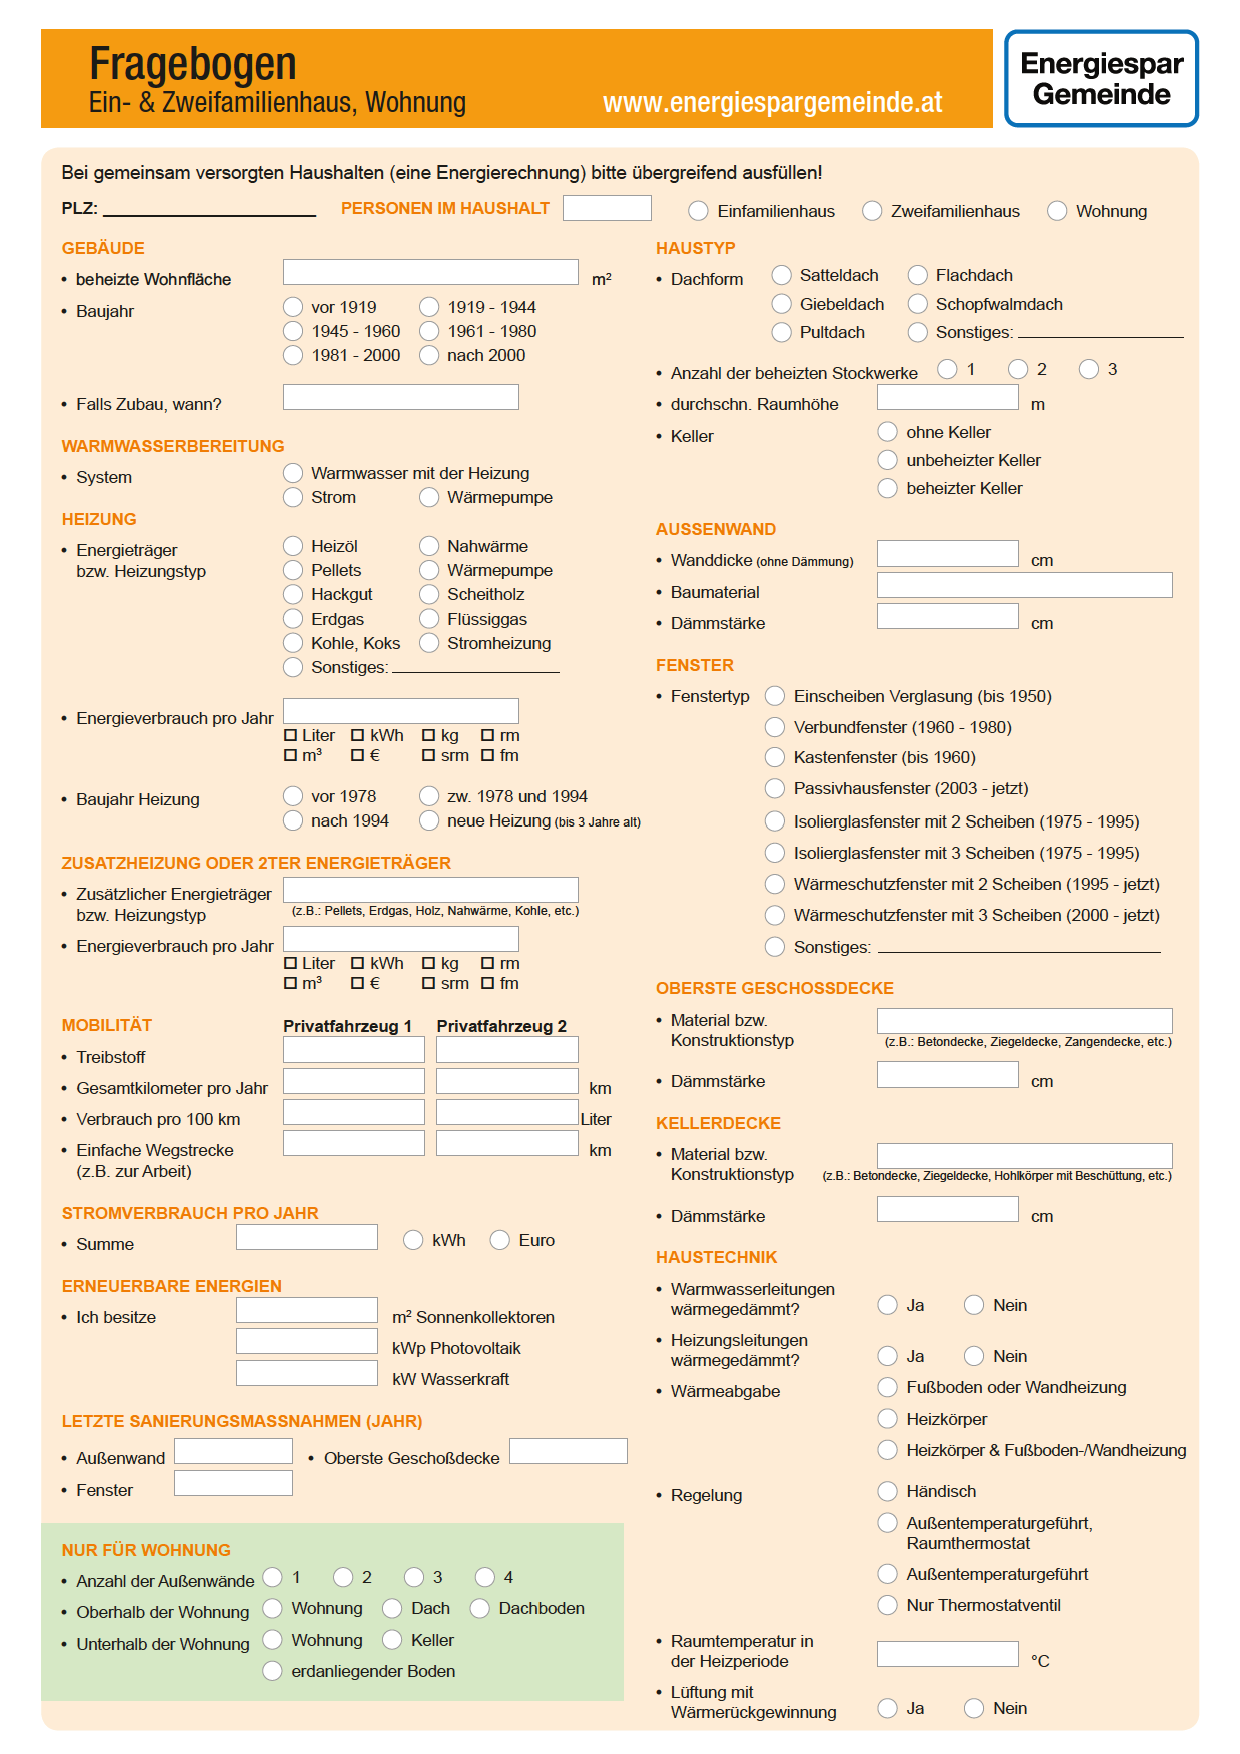
\includepdf[pages=1-,width=\textwidth,frame=true,pagecommand={}]{images/fragebogen}



